\documentclass[10pt]{beamer}
\usetheme{Feather}
\usepackage[T1]{fontenc}
\usepackage[utf8]{inputenc}
\usepackage[spanish]{babel}
\usepackage{mathrsfs}
\usepackage{amsmath}
\usepackage{amssymb}
\usepackage[utf8]{inputenc}
\usepackage[T1]{fontenc}
\usepackage{multirow}
\usepackage{multicol}
\usepackage{xcolor}
\usepackage{ragged2e}
 
\setbeamerfont{block body}{size=\small}
\title{Linear Algebra Library Junior C++ }
\subtitle{Algoritmos y Estructuras de Datos}
\author{Santiago Lopez, Oscar Velasco y Juanita Gómez}
\begin{document}
{\1
\begin{frame}[plain,noframenumbering]
  \titlepage 
\end{frame}}
%% 1
\begin{frame}{Problem Description}
\begin{itemize}
\item Difficulty to represent and perform operations between mathematical objects, such as vectors and  matrices. 

\end{itemize}
\center 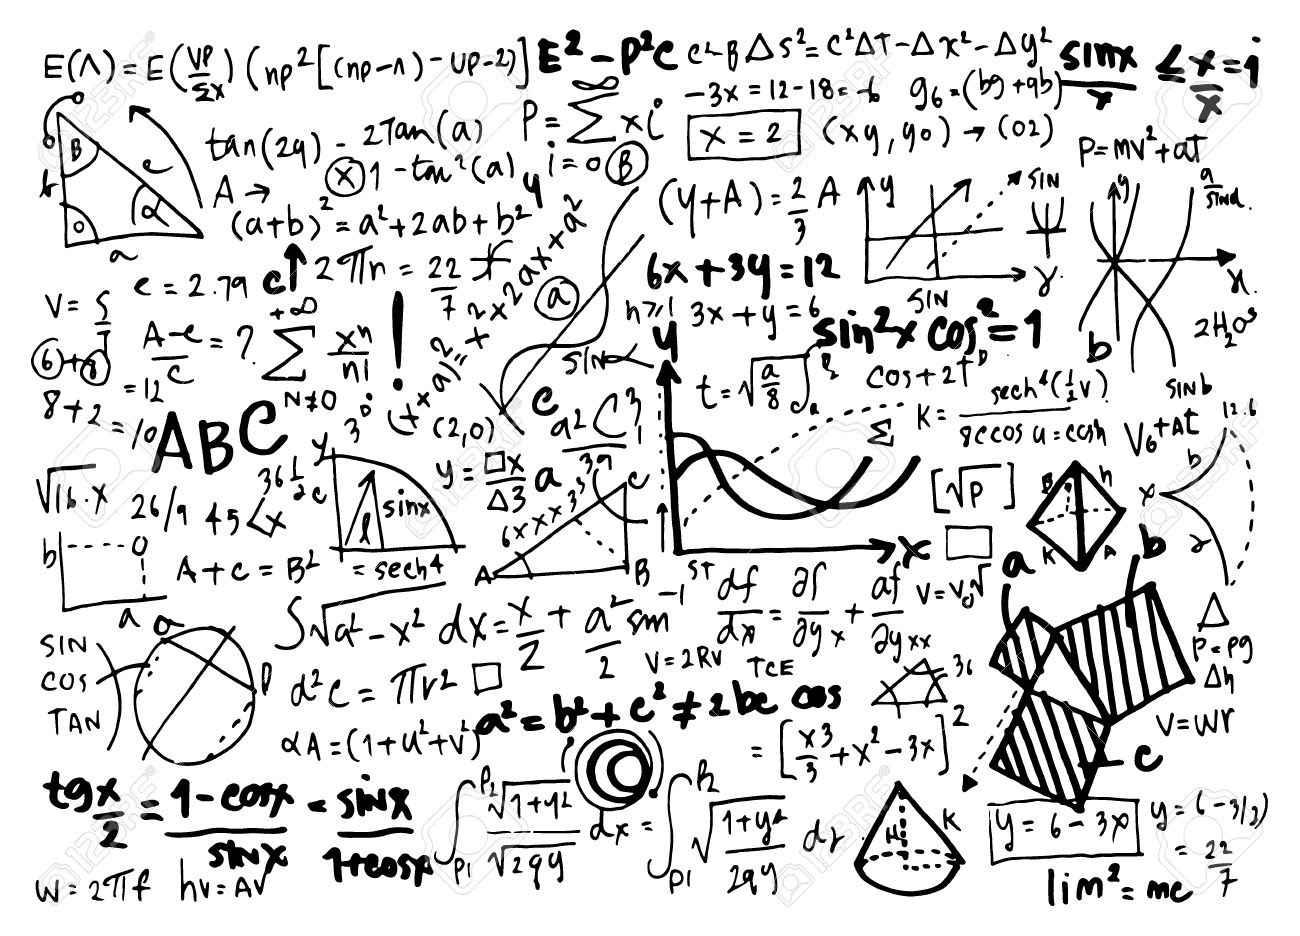
\includegraphics[scale=0.18]{LA.jpeg}
\end{frame}

\begin{frame}{Solution}
\begin{block}{}
Implementation of a basic linear algebra library with classes \textbf{Cvector} and \textbf{Cmatrix}
\end{block}
\begin{multicols}{2}
\center
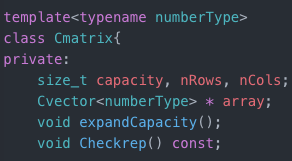
\includegraphics[scale=0.2]{Matrix}
\center
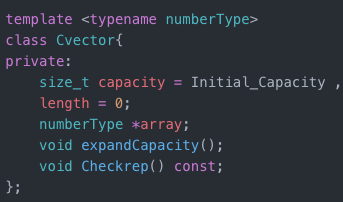
\includegraphics[scale=0.2]{Vector}
\end{multicols}

\begin{multicols}{2}
\begin{enumerate}
    \item``push", ``insert", ``erase", ``clear"   
    \item  +, -, * and /
    \item ==, !=, $>$=, $<$=, $<$, $>$.
    \item Dot product, cross product
    \item norm, normalization
    \item angle and projections.
    \item Gram-Schmidt
    \item Transpose and Inverse.
    \item LUP and QR decompositions
    \item Determinant and Eigen values.
\end{enumerate}
\end{multicols}
\end{frame}

%% 2
\begin{frame}{Vector Operations}
\begin{block}{1. a) Dot Product}
\center
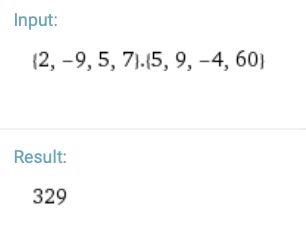
\includegraphics[scale=0.53]{1a.png}
\end{block}
\end{frame}
\begin{frame}{Vector Operations}
\begin{block}{1. b) Dot Product}
\center
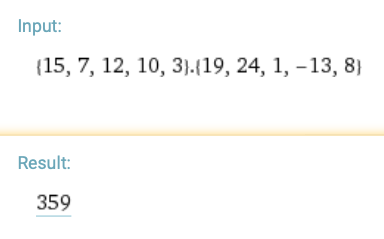
\includegraphics[scale=0.53]{1b.png}
\end{block}
\end{frame}
\begin{frame}{Vector Operations}
\begin{block}{2. a) Cross Product}
\center
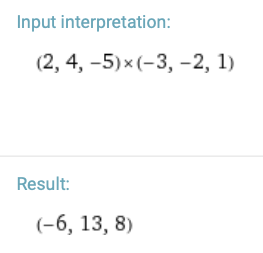
\includegraphics[scale=0.53]{2a.png}
\end{block}
\end{frame}
\begin{frame}{Vector Operations}
\begin{block}{2. b) Cross Product}
\center
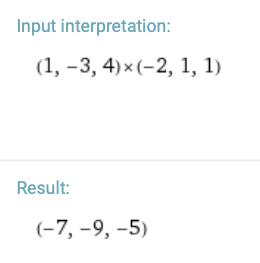
\includegraphics[scale=0.53]{2b.png}
\end{block}
\end{frame}
\begin{frame}{Vector Operations}
\begin{block}{3. a) Norm}
\center
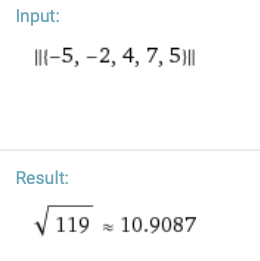
\includegraphics[scale=0.53]{3a.png}
\end{block}
\end{frame}
\begin{frame}{Vector Operations}
\begin{block}{3. b) Norm}
\center
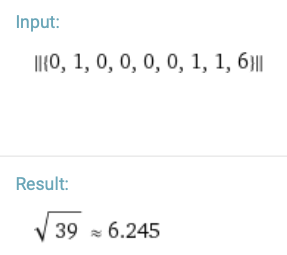
\includegraphics[scale=0.53]{3b.png}
\end{block}
\end{frame}
\begin{frame}{Vector Operations}
\begin{block}{4 a) Normalization}
\center
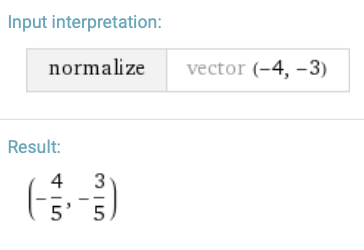
\includegraphics[scale=0.53]{4a.png}
\end{block}
\end{frame}
\begin{frame}{Vector Operations}
\begin{block}{4. b) Normalization}
\center
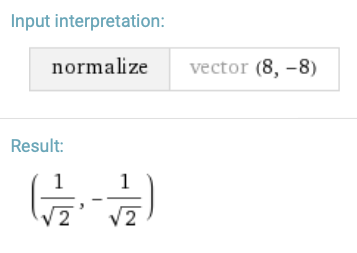
\includegraphics[scale=0.53]{4b.png}
\end{block}
\end{frame}
\begin{frame}{Vector Operations}
\begin{block}{5 a) Angle}
\center
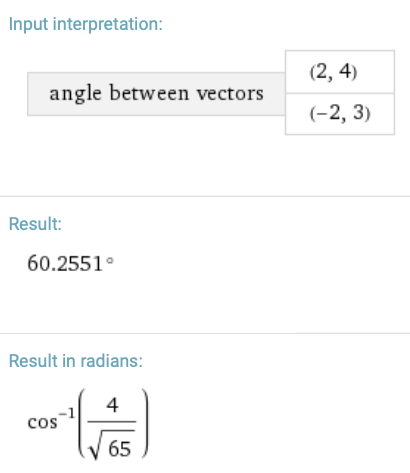
\includegraphics[scale=0.35]{5a.png}
\end{block}
\end{frame}
\begin{frame}{Vector Operations}
\begin{block}{5. b) Angle}
\center
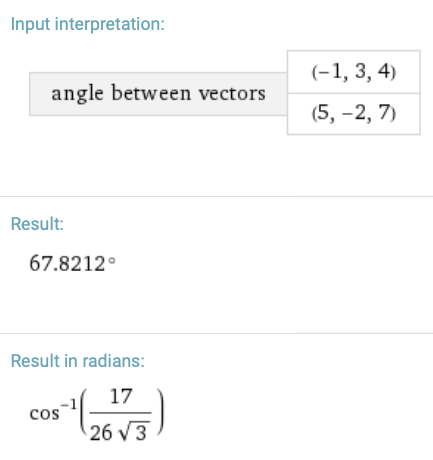
\includegraphics[scale=0.35]{5b.png}
\end{block}
\end{frame}
\begin{frame}{Vector Operations}
\begin{block}{6. a) Projection}
\center
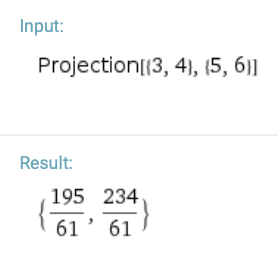
\includegraphics[scale=0.53]{6a.png}
\end{block}
\end{frame}

\begin{frame}{Vector Operations}
\begin{block}{6. b) Projection}
\center
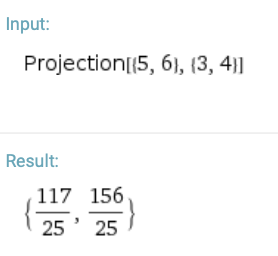
\includegraphics[scale=0.53]{6b.png}
\end{block}
\end{frame}


\begin{frame}{Vector Operations}
\begin{block}{7. Gram Schmidt}
\center
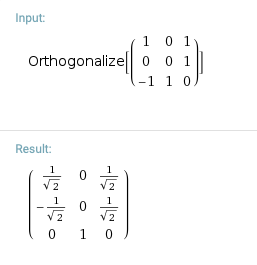
\includegraphics[scale=0.53]{GS.png}
\end{block}
\end{frame}
%%%%%%%%%%%%

\begin{frame}{Matrix Operations}
\begin{block}{1) Transpose}
\center
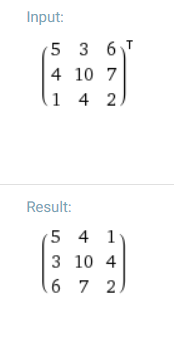
\includegraphics[scale=0.60]{1).png}
\end{block}
\end{frame}
\begin{frame}{Matrix Operations}
\includegraphics[scale=0.60]{M1.png}
\begin{block}{Some Basic Matrices}
\begin{itemize}
\item 2) Lower Triangular
\item 3) Upper Triangular
\end{itemize}
\end{block}
\end{frame}
\begin{frame}{Matrix Operations}
\begin{block}{Easy Matrices}
\begin{itemize}
\item 4) Identity 10 x 10 
\item 5) Null 4 x 5
\item 6) 1s Matrix 5 x 4
\item 7) Random Matrix
\end{itemize}
\end{block}
\end{frame}

\begin{frame}{Matrix Operations}
\includegraphics[scale=0.60]{M1.png}
\begin{block}{Modifiers}
\begin{itemize}
\item Swaps
\end{itemize}

\end{block}

\end{frame}

\begin{frame}{Matrix Operations}
\begin{block}{10) Determinant}
\center
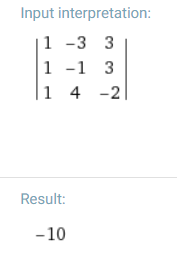
\includegraphics[scale=0.53]{10).png}
\end{block}
\end{frame}\begin{frame}{Matrix Operations}
\begin{block}{+}
\center
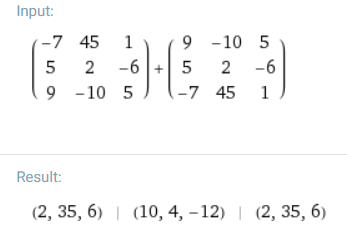
\includegraphics[scale=0.53]{+.png}
\end{block}
\end{frame}\begin{frame}{Matrix Operations}
\begin{block}{-}
\center
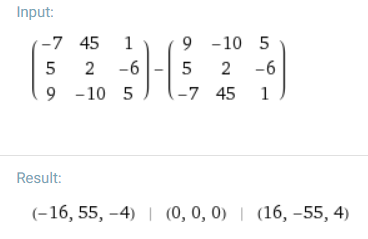
\includegraphics[scale=0.53]{-.png}
\end{block}
\end{frame}
\begin{frame}{Matrix Operations}
\begin{block}{Exponents}
\center
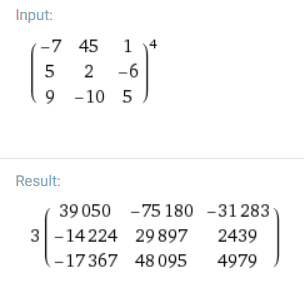
\includegraphics[scale=0.53]{^.png}
\end{block}
\end{frame}
\begin{frame}{Matrix Operations}
\begin{block}{Matrix-Vector Multiplication}
\center
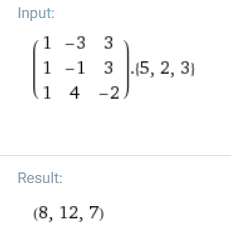
\includegraphics[scale=0.53]{*1.png}
\end{block}
\end{frame}
\begin{frame}{Matrix Operations}
\begin{block}{Vector-Matrix Multiplication}
\center
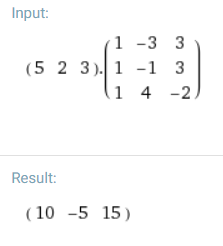
\includegraphics[scale=0.53]{*2.png}
\end{block}
\end{frame}
\begin{frame}{Matrix Operations}
\begin{block}{Matrix-Matrix Multiplication}
\center
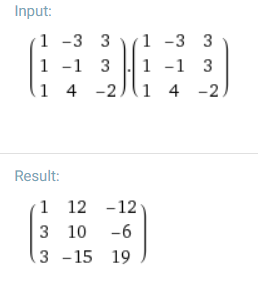
\includegraphics[scale=0.53]{*3.png}
\end{block}
\end{frame}
\begin{frame}{Matrix Operations}
\begin{block}{Exponentiation}
\center
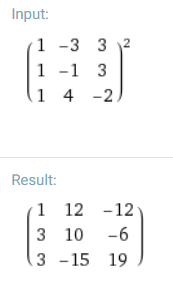
\includegraphics[scale=0.53]{*4.png}
\end{block}
\end{frame}
\begin{frame}{Matrix Operations}
\begin{block}{12) Inverse}
\center
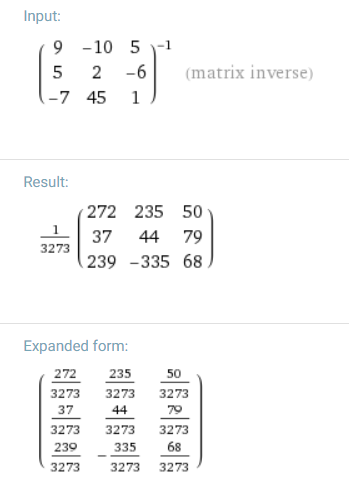
\includegraphics[scale=0.53]{12).png}
\end{block}
\end{frame}
\begin{frame}{Matrix Operations}
\begin{block}{13) QR Decomposition}
\center
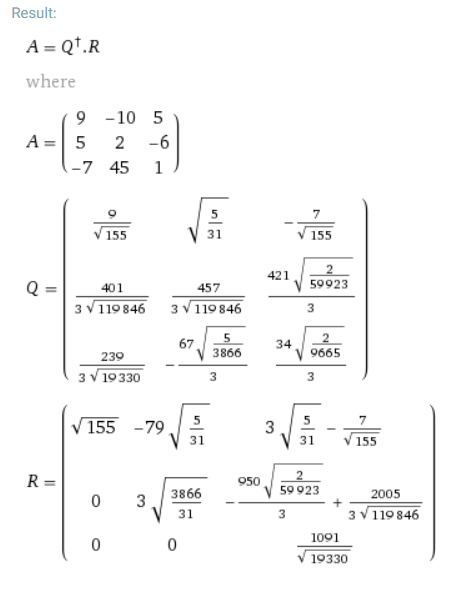
\includegraphics[scale=0.53]{QR.png}
\end{block}
\end{frame}
\begin{frame}{Matrix Operations}
\begin{block}{14) LU Decomposition}
\center
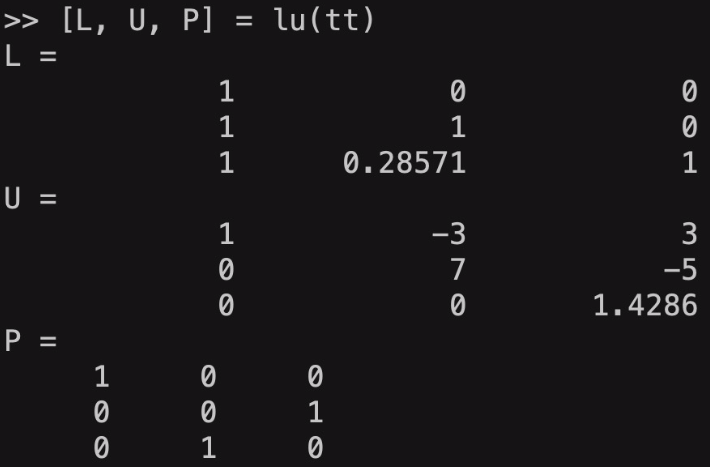
\includegraphics[scale=0.25]{LU.png}
\end{block}
\end{frame}
\begin{frame}{Matrix Operations}
\begin{block}{15) Eigen Values}
\center
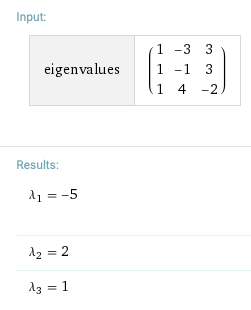
\includegraphics[scale=0.53]{EV}
\end{block}
\end{frame}
\begin{frame}{Challenges}
\begin{itemize}
\item Templates
\item Data Conversion
\item Computational Complexity
\item Objects Structure
\end{itemize}

\includegraphics[scale=0.3]{W.jpg}
\end{frame}
\begin{frame}{What is next?}
\begin{itemize}
\item Generalization for non-square matrixes
\item Easy Vector and Matrix Constructors
\item Reduce Computational Complexity 
\end{itemize}
\end{frame}

\end{document}





%%%%%% \include